\begin{document}

\def\title{Worksheet 4}

\newcommand{\qitem}{\qpart\item}

\renewcommand{\labelenumi}{(\alph{enumi})} % change default enum format to (a)
\renewcommand{\theenumi}{(\alph{enumi})} % fix reference format accordingly.
\renewcommand{\labelenumii}{\roman{enumii}.} % second level labels.
\renewcommand{\theenumii}{\roman{enumii}.}

\maketitle

\vspace{0.5em}

\begin{qunlist}

\input{\bank/discretization/mechanical_discretization.tex}
\newpage
% Authors: Taejin Hwang
% Emails: taejin@berkeley.edu

\qns{System Identification}

In this question, we will take a look at how to \textbf{identify} a system by taking experimental data taken from a (presumably) linear system to learn a discrete-time linear model for it using the least-squares.

Recall that a \textbf{linear, continuous-time,} system can be put in state-space form:
\begin{equation}
\ddt{}{t} \vec{x}(t) = A \vec{x}(t) + \vec{b} u(t)
\end{equation}

Now let's say we have an \textbf{unknown} linear system in which we can give an input $u(t)$ and observe the output $\vec{x}(t).$ We can model the system using the following diagram:
\begin{center}
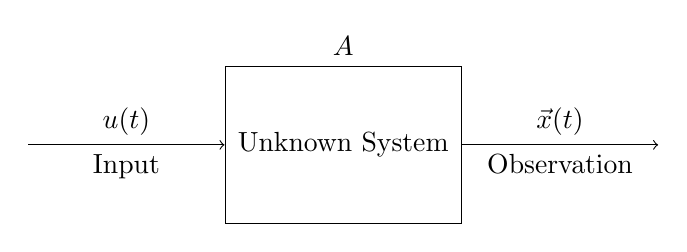
\begin{tikzpicture}
\node[draw, rectangle, minimum width = 3 cm, minimum height = 2 cm] (fl) at (0,0) {Unknown System};
\node[above] at (fl.north) {$A$};
\draw[<-] (fl) -- node[above]{$u(t)$} node[below]{Input} ++(-4,0);
\draw[->] (fl) -- node[above]{$\vec{x}(t)$} node[below]{Observation} ++(4,0);
\end{tikzpicture}
\end{center}

Recall from discussion that if we put a \textbf{piecewise constant} input $u(t) = u(i)$ for $t \in [i, i+1),$ then we can observe the output $\vec{x}(t)$ at time $t = i + 1,$ and form a discretized model of the observation.

\begin{center}
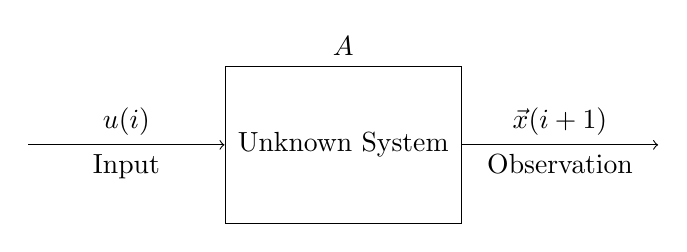
\begin{tikzpicture}
\node[draw, rectangle, minimum width = 3 cm, minimum height = 2 cm] (fl) at (0,0) {Unknown System};
\node[above] at (fl.north) {$A$};
\draw[<-] (fl) -- node[above]{$u(i)$} node[below]{Input} ++(-4,0);
\draw[->] (fl) -- node[above]{$\vec{x}(i + 1)$} node[below]{Observation} ++(4,0);
\end{tikzpicture}
\end{center}

\textbf{If} we knew the system, the relationship between $\vec{x}(i+1), \vec{x}(i),$ and $u(i)$ would be:
\begin{equation}
\vec{x}(i + 1) = A \vec{x}(i) + \vec{b} u(i)
\end{equation}

While this relation is useful, we currently do not know what the $A$ matrix or $\vec{b}$ vector are.

Therefore, we will start by creating unknown variables for the $A$ matrix, and $\vec{b}$ vector:
\begin{equation}
A = \begin{bmatrix} a_{11} & a_{12} \\ a_{21} & a_{22} \end{bmatrix} \ \ \text{and} \ \ \vec{b} = \begin{bmatrix} b_{1} \\ b_{2} \end{bmatrix}
\end{equation}
For the purposes of this question, we will be in the space $\mathbb{R}^2.$

\clearpage

\begin{enumerate}
  \qitem Let's say the system initially started at $\vec{x}(0) = \begin{bmatrix} x_{1}(0) \\ x_{2}(0) \end{bmatrix},$ and we gave an input at time $t = 0, \ u(0).$
  At time $t = 1,$ we observe $\vec{x}(1) = \begin{bmatrix} x_{1}(1) \\ x_{2}(1) \end{bmatrix}.$
  \textbf{How can you uncouple this matrix/vector equation into a system of linear equations?}

  \ws{\vspace{100px}}

  \sol {
    We start by writing out the matrix/vector equation for our unknown system:
    \begin{equation}
    \vec{x}(1) = \begin{bmatrix} x_{1}(1) \\ x_{2}(1) \end{bmatrix} = A \vec{x}(0) + \vec{b} u(0) =
    \begin{bmatrix} a_{11} & a_{12} \\ a_{21} & a_{22} \end{bmatrix} \begin{bmatrix} x_{1}(0) \\ x_{2}(0) \end{bmatrix} +
    \begin{bmatrix} b_{1} \\ b_{2} \end{bmatrix} u(0)
    \end{equation}

    Uncoupling these equations, we get:
    \pagebreak[0]
    \begin{gather*}
    x_{1}(1) = a_{11} x_{1}(0) + a_{12} x_{2}(0) + b_{1} u(0) \\
    x_{2}(1) = a_{21} x_{1}(0) + a_{22} x_{2}(0) + b_{2} u(0)
    \end{gather*}
  }

  \qitem Based on the system of linear equations created in the previous part, \textbf{how many unknown} variables do we have? Also, if we have a system of linear equations with $n$ unknown variables, at the minimum, \textbf{how many equations} would we need to solve our system?

  \ws{\vspace{100px}}

  \sol {
    The unknowns in this system of linear equations are: $a_{11}, a_{12}, a_{21}, a_{22}, b_{1}, b_{2}.$ \vskip 1pt
    If we have a system of linear equations with $n$ unknown variables, we will need at least $n$ equations to solve the system.
  }

  \qitem We now give another input at $t = 1, \ u(1),$ and observe $\vec{x}(2).$ \vskip 1pt
  \textbf{How many more equations do we get from this observation?}
  Also, how many more inputs will we need to observe until we have enough equations?

  \ws{\vspace{100px}}

  \sol {
    We can write out a similar observation as the one made in part(a):
    \begin{equation}
    \vec{x}(2) = \begin{bmatrix} x_{1}(2) \\ x_{2}(2) \end{bmatrix} = A \vec{x}(1) + \vec{b} u(1) =
    \begin{bmatrix} a_{11} & a_{12} \\ a_{21} & a_{22} \end{bmatrix} \begin{bmatrix} x_{1}(1) \\ x_{2}(1) \end{bmatrix} +
    \begin{bmatrix} b_{1} \\ b_{2} \end{bmatrix} u(1)
    \end{equation}

    Uncoupling these equations again, we will get:
    \pagebreak[0]
    \begin{gather*}
    x_{1}(2) = a_{11} x_{1}(1) + a_{12} x_{2}(1) + b_{1} u(1) \\
    x_{2}(2) = a_{21} x_{1}(1) + a_{22} x_{2}(1) + b_{2} u(1)
    \end{gather*}
    Notice that for every observation we make at a given time step, we will get $2$ more equations.
    This means we will have to look at a total of $3$ time steps to get $6$ equations.
    Taking the initial condition $\vec{x}(0)$ into account, we will have to observe a total of $4$ inputs.
  }

  \qitem Assuming we have taken all of the necessary measurements of $x(t)$ at time $t = 0, 1, 2, ...$ \vskip 1pt
  \textbf{How can we set up our system of linear equations as a matrix-vector equation?}

  \ws{\vspace{100px}}

  \sol {
    We can set up the following system of linear equations:
    $$
    \begin{bmatrix}
    x_{1}(0) & x_{2}(0) & u(0) & 0 & 0 & 0 \\
    x_{1}(1) & x_{2}(1) & u(1) & 0 & 0 & 0 \\
    x_{1}(2) & x_{2}(2) & u(2) & 0 & 0 & 0 \\
    0 & 0 & 0 & x_{1}(0) & x_{2}(0) & u(0) \\
    0 & 0 & 0 & x_{1}(1) & x_{2}(1) & u(1) \\
    0 & 0 & 0 & x_{1}(2) & x_{2}(2) & u(2)
    \end{bmatrix}
    \begin{bmatrix} a_{11} \\ a_{12} \\ b_{1} \\ a_{21} \\ a_{22} \\ b_{2} \end{bmatrix}
    = \begin{bmatrix} x_{1}(1) \\ x_{1}(2) \\ x_{1}(3) \\ x_{2}(1) \\ x_{2}(2) \\ x_{2}(3) \end{bmatrix}$$
    This can be written in as a matrix vector equation $D \vec{s} = \vec{y}$ and we can solve for $\vec{s} = D^{-1} \vec{y}$
  }

  \qitem While we can set up a matrix vector equation and uniquely solve our system, the output of the system can be noisy.
  Therefore, we update our model by considering a noise term $w(i)$ at time $t = i.$
  \begin{equation}
    \vec{x}(i + 1) = A \vec{x}(i) + \vec{b} u(i) + w(i)
  \end{equation}
  How can we set up a system of equations in a similar fashion but with a noise vector $\vec{w}?$
  \begin{equation}
    \vec{y} = D \vec{s} + \vec{w}
  \end{equation}

  \ws{\vspace{100px}}

  \sol {
    $$
    \begin{bmatrix} x_{1}(1) \\ x_{1}(2) \\ x_{1}(3) \\ x_{2}(1) \\ x_{2}(2) \\ x_{2}(3) \end{bmatrix}
    =
    \begin{bmatrix}
    x_{1}(0) & x_{2}(0) & u(0) & 0 & 0 & 0 \\
    x_{1}(1) & x_{2}(1) & u(1) & 0 & 0 & 0 \\
    x_{1}(2) & x_{2}(2) & u(2) & 0 & 0 & 0 \\
    0 & 0 & 0 & x_{1}(0) & x_{2}(0) & u(0) \\
    0 & 0 & 0 & x_{1}(1) & x_{2}(1) & u(1) \\
    0 & 0 & 0 & x_{1}(2) & x_{2}(2) & u(2)
    \end{bmatrix}
    \begin{bmatrix} a_{11} \\ a_{12} \\ b_{1} \\ a_{21} \\ a_{22} \\ b_{2} \end{bmatrix}
    + \begin{bmatrix} w(0) \\ w(1) \\ w(2) \\ w(0) \\ w(1) \\ w(2) \end{bmatrix} $$
  }

  \qitem We can try to solve our system of equations, but we do not know what $\vec{w}$ is. \vskip 1pt
  What we can do however, is to take more measurements, and set up a \textbf{least squares} problem as seen in 16A.
  What would the least squares problem be if we took measurements up to time step $t = 5?$

  \ws{\vspace{100px}}

  \sol {
  $$
    \begin{bmatrix} x_{1}(1) \\ x_{1}(2) \\ x_{1}(3) \\ x_{1}(4) \\ x_{1}(5) \\ x_{2}(1) \\ x_{2}(2) \\ x_{2}(3) \\ x_{2}(4) \\ x_{2}(5) \end{bmatrix}
    =
    \begin{bmatrix}
    x_{1}(0) & x_{2}(0) & u(0) & 0 & 0 & 0 \\
    x_{1}(1) & x_{2}(1) & u(1) & 0 & 0 & 0 \\
    x_{1}(2) & x_{2}(2) & u(2) & 0 & 0 & 0 \\
    x_{1}(3) & x_{2}(3) & u(3) & 0 & 0 & 0 \\
    x_{1}(4) & x_{2}(3) & u(4) & 0 & 0 & 0 \\
    0 & 0 & 0 & x_{1}(0) & x_{2}(0) & u(0) \\
    0 & 0 & 0 & x_{1}(1) & x_{2}(1) & u(1) \\
    0 & 0 & 0 & x_{1}(2) & x_{2}(2) & u(2) \\
    0 & 0 & 0 & x_{1}(3) & x_{2}(3) & u(3) \\
    0 & 0 & 0 & x_{1}(4) & x_{2}(4) & u(4)
    \end{bmatrix}
    \begin{bmatrix} a_{11} \\ a_{12} \\ b_{1} \\ a_{21} \\ a_{22} \\ b_{2} \end{bmatrix}
    + \begin{bmatrix} w(0) \\ w(1) \\ w(2) \\ w(0) \\ w(1) \\ w(2) \end{bmatrix} $$

    Which can equivalently be written as:
    \begin{equation}
      \vec{y} = D \vec{s} + \vec{w}
    \end{equation}
    For the least squares problem, we will want to minimize $\norm{\vec{w}}_{2} = \norm{y - D \vec{s}}_{2}$
    }

  \qitem How would we solve this least squares problem?

  \ws{\vspace{100px}}

  \sol {
    Recall from 16A that if we are given the least squares problem:
    \begin{equation}
      A \vec{x} = \vec{b} + \vec{e}
    \end{equation}
    The solution that minimizes the norm of the residual $\norm{\vec{e}}_{2}$ is:
    \begin{equation}
      \vec{\hat{x}} = (A^{T} A)^{-1} A^{T} \vec{b}
    \end{equation}
    Therefore the solution to the least squares problem above will be:
    \begin{equation}
      \vec{\hat{s}} = (D^{T} D)^{-1} D^{T} \vec{y}
    \end{equation}
    The $\vec{\hat{s}}$ will give the best possible estimate for the $A$ and $\vec{b}.$
  }
\end{enumerate}

% \qitem Explain why the system
%     \begin{align*}
%         \ddt{x}{t} &= ax + by \\
%         \ddt{y}{t} &= cx + dy
%     \end{align*}
%     can be equivalently formulated as
%     \[
%         \ddt{}{t} \begin{bmatrix} x \\ y \end{bmatrix} = \begin{bmatrix} a & b \\ c & d \end{bmatrix} \begin{bmatrix} x \\ y \end{bmatrix}
%     \]


% \qitem Given the following system:
%     \begin{align*}
%         \ddt{x}{t} &= x \\
%         \ddt{y}{t} &= y
%     \end{align*}

%     With initial conditions $x(0) = x_0, \ y(0) = y_0,$

%     \begin{enumerate}
%         \qitem What is an appropriate state vector for this system?
%         \qitem What is the initial condition of this system?
%         \qitem Convert this system into its State-space representation.
%         \qitem How can you solve for $x(t)$ and $y(t)?$
%     \end{enumerate}

\newpage
% Authors: Akash Velu, Shreyas Krisnaswamy
% Emails: akashvelu@berkeley.edu, shrekris@berkeley.edu

\qns{Aperture Stability}

As an intern at Aperture Laboratories, it is your job to make sure the robots being built are stable systems.
As a reminder, if the following conditions are met the system will be stable:

\begin{itemize}

\item For discrete time systems of the form:
\begin{equation}
\vec{x}[t+1] = A\vec{x}[t] + Bu[t] + \vec{w}[t]
\end{equation}
All eigenvalues of the matrix A, $\lambda_{i},$ have magnitude $|\lambda_{i}| < 1.$

\item For continuous time systems of the form:
\begin{equation}
\ddt{}{t} \vec{x}[t] = A\vec{x}[t] + Bu[t] + \vec{w}[t]
\end{equation}
All eigenvalues of the matrix A, $\lambda_{i},$ have real part $\mathfrak{Re}(\lambda_{i})< 0.$
\end{itemize}

\begin{enumerate}

\qitem According to your boss, the first robot, GLaDOS, can be described with the following discrete time system:
\begin{equation*}
    \vec{x}[t+1] =
    \begin{bmatrix}
    \frac{3}{8} & \frac{1}{8}\\
    \frac{1}{8} & \frac{3}{8}\\
    \end{bmatrix}
    \vec{x}[t] +
    \begin{bmatrix}
    1\\
    0\\
    \end{bmatrix}
    u[t]
\end{equation*}

Is she stable?

\sol {
% \begin{align*}
% A\vec{v} &= \lambda\vec{v} \\
% A\vec{v} - \lambda\vec{v} &= 0 \\
% (A - \lambda{}I)\vec{v} &= 0 \\
% det(A - \lambda{}I) &= 0
% \end{align*}

\begin{align*}
\text{det} (A - \lambda{}I) &=
\text{det} \Big(
\begin{bmatrix}
\frac{3}{8} - \lambda{} & \frac{1}{8}\\
\frac{1}{8} & \frac{3}{8} - \lambda{}\\
\end{bmatrix} \Big) = \big(\frac{3}{8} - \lambda{}\big)\big(\frac{3}{8} - \lambda{}\big) - \big(\frac{1}{8}\big)\big(\frac{1}{8}\big) \\
&= \lambda{}^2 - \frac{3}{4}\lambda{} + \frac{1}{8} = \big(\lambda{} - \frac{1}{2}\big)\big(\lambda{} - \frac{1}{4}\big) = 0\\
\end{align*}
Therefore, we see that
$$
\lambda{} = \frac{1}{2}, \frac{1}{4}$$

Since the system is a discrete time system, and both eigenvalues have magnitude smaller than 1, GLaDOS is stable.
}

\qitem Your boss now gives you data on the P-body robot. Is she stable?
Her motion is described with the following discrete time system:
\begin{equation*}
    \vec{x}[t + 1] =
    \begin{bmatrix}
    -2 & -1\\
    1 & -2\\
    \end{bmatrix}
    \vec{x}[t] +
    \begin{bmatrix}
    1\\
    1\\
    \end{bmatrix}
    u[t]
\end{equation*}

\sol {
  \begin{align*}
    \text{det}(A - \lambda{}I) &= \Big(
    \begin{bmatrix}
    -2 - \lambda{} & -1\\
    1 & -2 - \lambda{}\\
    \end{bmatrix} \Big) = (-2 - \lambda{})(-2 - \lambda{}) - (-1)(1) \\
    &= \lambda{}^2 + 4\lambda{} + 5 = (\lambda{} - (-2 + j))(\lambda{} - (-2 - j)) = 0 \\
  \end{align*}
  Therefore we can compute the eigenvalues as
  $$\lambda{} = -2 \pm j$$
  However, the magnitude of both of these eigenvalues are $|\lambda| = \sqrt{5} \geq 1.$ Therefore, Atlas is unstable.
}

\qitem
Now your boss gives you data on a more advanced robot, Atlas.
Is he stable?
His movements can be described with the following continuous time system:
\begin{equation*}
    \frac{d}{dt}\vec{x}[t] =
    \begin{bmatrix}
    -2 & -1\\
    1 & -2\\
    \end{bmatrix}
    \vec{x}[t] +
    \begin{bmatrix}
    1\\
    1\\
    \end{bmatrix}
    u[t]
\end{equation*}

\sol{
  This is the exact same system as the previous system but in continuous time. The eigenvalues will be the same:
  $$\lambda{} = -2 \pm j$$
  This time, since this is a continuous time system, the conditions for stability have changed. Since $\mathfrak{Re}(\lambda) < 0$ for both eigenvalues, we conclude by saying that this system is stable.
}

\qitem Lastly, your boss gives you data on the Wheatley robot. Is he stable?
His motion is described with the following discrete time system:
\begin{equation*}
    \vec{x}[t+1] =
    \begin{bmatrix}
    \frac{\sqrt{3}}{2} & -\frac{1}{2}\\
    \frac{1}{2} & \frac{\sqrt{3}}{2}\\
    \end{bmatrix}
    \vec{x}[t] +
    \begin{bmatrix}
    0\\
    1\\
    \end{bmatrix}
    u[t]
\end{equation*}

\sol {
  You can also note that A is the rotation matrix, and make the observation that the eigenvalues are on the unit circle.
  Without even doing any calculations, we know Wheatley is unstable since $|\lambda| = 1.$

  This can also be realized by computing the eigenvalues in the following manner:
  \begin{align*}
    \text{det}(A - \lambda{}I) &= \text{det} \Big(
    \begin{bmatrix}
    \frac{\sqrt{3}}{2} - \lambda{} & -\frac{1}{2}\\
    \frac{1}{2} & \frac{\sqrt{3}}{2} - \lambda{}\\
    \end{bmatrix} \Big) = (\frac{\sqrt{3}}{2} - \lambda{})^{2} + \frac{1}{4} = \lambda{}^{2} - \sqrt{3} \lambda + 1 = 0
  \end{align*}
  Using the quadratic formula, we see that the eigenvalues are:
  $$\lambda = \frac{\sqrt{3}}{2} \pm \frac{1}{2} \sqrt{(-\sqrt{3})^{2} - 4 \cdot 1} = \frac{\sqrt{3}}{2} \pm \frac{1}{2}j$$

  Intuitively, you can see that this system is unstable since it will continue rotating and will never converge to a steady state.
}
\end{enumerate}

\newpage
\input{\bank/stability/graph_stability.tex}
\newpage
% Authors: Yi Zhao, Taejin Hwang
% Emails: taejin@berkeley.edu

\qns{System Feedback}

Consider the following continuous time system:
$$
\frac{d^2}{dt^2} x(t) = -x(t)
$$
We convert this system to state space form:

\begin{equation}
  \ddt{}{t} \vec{x}(t) = A \vec{x}(t) + B \vec{u}(t)
\end{equation}

We will pick our state variable $\vec{x} = \begin{bmatrix} x_1(t) \\ x_2(t) \end{bmatrix},$
with $x_1(t) = x(t)$ and $x_2(t) = \frac{d}{dt} x(t)$.

\begin{enumerate}

\qitem What are the values of the $A$ matrix?

\ws{
\vspace{30px}
}

\sol {
	$$
    A = \begin{bmatrix}
    0 & 1 \\
    -1 & 0
    \end{bmatrix}
    $$
}

% \qitem How about the matrix $B$ and the input vector $\vec{u}(t)?$

% \sol {
%   The current system can be modeled as:
%   \begin{equation}
%   \ddt{}{t} \vec{x}(t) = A \vec{x}(t)
%   \end{equation}
%   We do not have an input vector for the system, nor do we have a matrix $B.$ \vskip 1pt
%   We can treat them as zero, but the dimensions of $B$ and $\vec{u}(t)$ are currently undefined.
% }

\qitem Is this continuous time system stable? How would you describe its behavior?

\ws{
\vspace{50px}
}

\sol{
	The eigenvalues of the $A$ matrix will be $\pm j.$
  Since $\mathfrak{Re}(\lambda) = 0,$ and is not less than $0,$ the system is unstable.
  It can be described as an oscillatory system that never dies out.
}

\end{enumerate}

We want to change the behavior of the system using a feedback control model:
$$
\frac{d}{dt}
\begin{bmatrix}
x_1(t) \\
x_2(t)
\end{bmatrix}
=
A
\begin{bmatrix}
x_1(t) \\
x_2(t)
\end{bmatrix}
+
\begin{bmatrix}
0 \\
1
\end{bmatrix}
u(t)
$$
To do this, we set $u(t) = F\vec{x}(t)$, where $F = \begin{bmatrix} f_1 & f_2 \end{bmatrix}$. Note that $F$ is a $1 \times 2$ matrix.

\meta {
  In the generalized state-space model, $B$ is an $n \times p$ matrix and $\vec{u}$ will be a vector in $\mathbb{R}^{p}.$ Therefore, since $\vec{u} = F \vec{x},$ and $\vec{x}$ is in $\mathbb{R}^{n},$ our $F$ matrix in the general state-space model will be of size $p \times n.$
}

\begin{enumerate}[resume]
\qitem We will now try to use our knowledge of controllability to stabilize this system. Is this continuous time system controllable?

\ws{
\vspace{50px}
}

\meta {
  Make sure to emphasize that we can only pick every eigenvalue of the system if it is controllable.
  We can also make an unstable system stable, if we can control all of the unstable eigenvalues, but we would not be able to control \textbf{every} eigenvalue for the system.
}

\sol{
  We can compute our controllability matrix as
  $$\mathcal{C} = \begin{bmatrix} \vec{b} & A \vec{b} \end{bmatrix} =
  \begin{bmatrix}
  0 & 1 \\
  1 & 0
  \end{bmatrix}$$
  This controllability matrix is full-rank since its columns are linearly independent, so the system is controllable.
}

\item After plugging in our input, $u(t) = F\vec{x}(t),$ what will our new system be? How can you write out this system of differential equations in matrix/vector form?

\ws{
\vspace{100px}
}

\sol {
  We know that our $B$ matrix is: $\begin{bmatrix} 0 \\ 1 \end{bmatrix}$ and our input $u(t) = f_1 x_1(t) + f_2 x_2(t).$ \vskip 1pt
  If we plug this into our system, we will get:
  \begin{equation}
    \ddt{}{t} \vec{x}(t) =
    \begin{bmatrix}
    0 & 1 \\
    -1 & 0
    \end{bmatrix}
    \begin{bmatrix} x_1(t) \\ x_2(t) \end{bmatrix} +
    \begin{bmatrix}
    0 & 0 \\
    f_1 & f_2 \\
    \end{bmatrix}
    \begin{bmatrix} x_1(t) \\ x_2(t) \end{bmatrix}
  \end{equation}

  This means our new system will be:
  \begin{equation}
    \ddt{}{t} \vec{x}(t) =
    \begin{bmatrix}
    0 & 1 \\
    -1 + f_1 & f_2
    \end{bmatrix}
    \begin{bmatrix} x_1(t) \\ x_2(t) \end{bmatrix}
  \end{equation}
  We can alternatively represent this as a matrix/vector system of differential equations:
  \begin{equation}
    \ddt{}{t} \vec{x}(t) = (A + BF) \vec{x}(t)
  \end{equation}
}

\qitem We will define the new matrix derived in the previous part as $A_{cl}$ for the closed loop system.
What are the eigenvalues of this new matrix $A_{cl}?$

\ws{
\vspace{125px}
}


\sol {
  We first compute the characteristic polynomial of $A_{cl}.$
  $$\text{det}(A_{cl} - \lambda I) =
  \text{det}
  \bigg(
  \begin{bmatrix}
    -\lambda & 1 \\
    -1 + f_1 & f_2 - \lambda
  \end{bmatrix}
  \bigg) = \lambda(\lambda - f_2) - 1(-1 + f_1) = \lambda^{2} - f_2 \lambda + 1 - f_1$$
  The eigenvalues will be the roots of this characteristic polynomial:
  $$\lambda = \frac{f_2}{2} \pm \frac{1}{2} \sqrt{f_2^{2} - 4(1 - f_1)}$$
}

\qitem Suppose $f_1 = 1$ and $f_2 = 2,$ what will the eigenvalues of this system be?
How about when $f_1 = -1$ and $f_2 = -2$?

\ws{
\vspace{125px}
}


\sol{
	If $f_1 = 1$ and $f_2 = 2,$ then the eigenvalues will be:
  $$1 \pm \frac{1}{2} \sqrt{4 - 4(1 - 1)} = 0, \ 2$$
  Since both of the eigenvalues have $\mathfrak{Re}(\lambda) = 0, 2 >= 0,$ this system will be unstable.

  Now suppose $f_1 = -1$ and $f_2 = -2,$ then the eigenvalues will be:
  $$-1 \pm \frac{1}{2} \sqrt{4 - 4(1 + 1)} = -1 \pm j$$
  Since $\mathfrak{Re}(\lambda) = -1 < 0,$ for both eigenvalues, this system will be stable.
}

\qitem What values of $f_1$ and $f_2$ will remove the oscillatory behavior completely and still stabilize the system?

\ws{
\vspace{75px}
}


\meta{
Have students sketch out/visualize and understand what varying k do to the eigenvalues.
}

\sol{
	To remove oscillatory behavior, and stabilize the system, the square root term $\sqrt{f_2^{2} - 4(1 - f_1)}$ must be positive, and the real part of both eigenvalues must be less than 0.

	As example of this would be $f_1 = -1$ and $k_ 2 = -3.$
  This gives the system eigenvalues of $-1$ and $-2$ while removing oscillatory behavior and being stable.
}

\end{enumerate}

\newpage
% % Author: Taejin Hwang
% Email: taejin@berkeley.edu

\qns{Controlling a System}

We are given a discrete time state space system, where $\vec{x}$ is our \textbf{state vector}, $A$ is the \textbf{state space model} of the system, $B$ is the \textbf{input matrix}, and $\vec{u}$ is the \textbf{control input vector}.
\begin{equation}
\vec{x}[t + 1] = A \vec{x}[t] + B\vec{u}[t]
\end{equation}
We define a system to be controllable if: \textbf{given a set of inputs, we can move the system from any initial state to any final state by choosing a sequence of inputs.} This has an important physical meaning; if a physical system is controllable, that means that we can get anywhere in the state space. For example, if a robot is controllable, it is able to travel anywhere in the system it is living in (given enough time and control inputs).

\textbf{We will start with the assumption that the system started at rest at the zero vector: $\vec{x}[0] = \vec{0}$}, and our state space will be an n-dimensional vector in $\mathbb{R}^{n}.$ 

\begin{enumerate}

\qitem \textbf{How can you write out $\vec{x}[1]$ using the state space equation? How about $\vec{x}[2]?$}

\ws{\vspace{75px}}
\sol {
  Using the state space model $\vec{x}[i + 1] = A \vec{x}[i] + B \vec{u}[i],$
  $$\vec{x}[1] = A \vec{x}[0] + B \vec{u}[0] = A \vec{0} + B \vec{u}[0] = B \vec{u}[0]$$
  At time step $t = 2,$
  $$\vec{x}[2] = A \vec{x}[1] + B \vec{u}[1] = A (B \vec{u}[0]) + B \vec{u}[1]$$
}

\qitem \textbf{Given these two observations and the initial condition $\vec{x}[0] = \vec{0}$, where can $\vec{x}$ reach in our state space reach after 2 time steps (i.e. at $t = 2$)?}
\ws{\vspace{100px}}
\sol {
  From the previous part, we know that
  $$\vec{x}[2] = A (B \vec{u}[0]) + B \vec{u}[1] = AB \vec{u}[0] + B \vec{u}[1]$$
  Let's say $B$ has two columns, although we can generalize this for any number of columns. \vskip 1pt
  We can then equivalently write out our equation as:
  $$\vec{x}[2] = \begin{bmatrix} A \vec{b}_{1} & A \vec{b}_{2} \end{bmatrix} \begin{bmatrix} u_{1}[0] \\ u_{2}[0] \end{bmatrix} + 
  \begin{bmatrix} \vec{b}_{1} & \vec{b}_{2} \end{bmatrix} \begin{bmatrix} u_{1}[1] \\ u_{2}[1] \end{bmatrix} = 
  u_{1}[0] A \vec{b}_{1} + u_{2}[0] A \vec{b}_{2} + u_{1}[1] \vec{b}_{1} + u_{2}[1] \vec{b}_{2}.$$
  Since $\vec{u}$ is a vector we have full control over, we can reach anywhere in:
  $$\text{span}(A \vec{b}_{1}, A \vec{b}_{2}, \vec{b}_{1}, \vec{b}_{2})$$
  In general, we could reach anywhere in the span of the columns of $B$ and $AB.$
}

\qitem \textbf{Given $n$ observations, where in our state space can $\vec{x}$ reach at time $t = n?$}
\ws{\vspace{100px}}
\sol {
  We will start off in a similar manner by writing out $\vec{x}(3)$ in terms of $\vec{x}[2]$ and $\vec{u}[2].$
  $$\vec{x}(3) = A \vec{x}[2] + B \vec{u}[2] =  A (AB \vec{u}[0] + B \vec{u}[1]) + B \vec{u}[2] = A^2 B \vec{u}[0] + AB \vec{u}[1] + B \vec{u}[2].$$
  Using a similar argument as the previous part, we will see that we can reach anywhere in the span of the columns of $B, \ AB, \ A^{2} B.$ We can continue doing this, and see that after $n$ time steps,
  \begin{align*}
  \vec{x}[i] &= A \vec{x}[i - 1] + B \vec{u}[i - 1] \\
  &= A^{n - 1}B \vec{u}[0] + A^{n - 2}B \vec{u}[1] + A^{n - 3}B \vec{u}[2] + \cdots + AB \vec{u}[i - 2] + B \vec{u}[i - 1]
  \end{align*}
  Therefore, after $n$ timesteps, we can reach anywhere in the span of the columns of $\{ B, \ AB, \ A^2 B, \cdots, A^{n-1} B \}.$
}

\qitem \textbf{Show that if the columns of $A^{k} B$ are linearly dependent, then the columns of $A^{k + 1} B$ are also linearly dependent.}
\ws{\vspace{100px}}
\meta {
  Make sure your students understand the reason for proving this. We want to be able to define a \textit{finite} controllability matrix to check if a system is controllable. If we don't prove that we only need to check up to $A^{n - 1}B$, then there's no guarantee that some infinitely large controllability matrix may end up having rank $n$.
}
\sol {
  We first make the observation that the columns of $A^{k} B$ are:
  $$A^{k} B = \begin{bmatrix} A^{k} \vec{b_1} & A^{k} \vec{b_2} & \cdots & A^{k} \vec{b_m} \end{bmatrix}$$
  Where $\vec{b}_{i}$ is the $i^{th}$ column of the matrix $B.$ \vskip 1pt
  Now let's suppose that the columns of $A^{k} B$ are linearly dependent. 
  We can say that if we have scalars $\alpha_i$ such that 
  $$\alpha_{1} A^{k} \vec{b_1} + \cdots + \alpha_{m} A^{k} \vec{b_m} = \vec{0},$$
  then at least one of the $\alpha_i$ must be nonzero. Now if we left multiply by $A,$ we see that:
  $$A(\alpha_{1} A^{k} \vec{b_1} + \cdots + \alpha_{m} A^{k} \vec{b_m}) = \alpha_{1} A^{k+1} \vec{b_1} + \cdots + \alpha_{m} A^{k+1} \vec{b_m} = \vec{0}.$$ 
  As a result, we observe that if we have a linear combination of the columns of $A^{k + 1} B$ equal to the zero vector, at least one of the scalars is nonzero. This shows that the columns of $A^{k + 1} B$ must be linearly dependent.
}

\qitem To summarize our work from the previous parts, we now define a controllability matrix

\meta {
  This is definitely the most difficult part of the question. 
  The previous parts were more or less intuitive, but here students will have to think about how part (d) relates to "redundant" measurements.
}

\begin{equation}
\mathcal{C} = \begin{bmatrix} B & AB & A^2B & \cdots & A^{n-2}B & A^{n-1}B \end{bmatrix}
\end{equation}
\textbf{Based on the previous parts, when can we say our system is controllable? (i.e. we can reach anywhere in our state space using our system)}

\sol {
  Using our knowledge from part (c), we can say that $\vec{x}$ can reach anywhere in the span of the columns of $\mathcal{C}$ after $n$ time steps. 
  We also saw in part (d), that if $A^{k}B$ had linearly dependent columns, then $A^{k + 1}B$ will also have linearly dependent columns. \vskip 1pt
  This means if one of our measurements at time $t = k,$ was linearly dependent from our previous measurements, then the future measurements $t = k + 1$ onward, will also be linearly dependent from the previous ones. In other words, every redundant measurement taken after a redundant one will continue to be redundant. \vskip 1pt
  We must take at least $n$ measurements, since we want to span all of $\mathbb{R}^n,$ and $B$ may just be a single vector.
  Therefore, we conclude by saying that our system can reach anywhere in our state-space, $\mathbb{R}^{n},$ if $\mathcal{C}$ is a matrix of rank $n.$ \vskip 1pt
  This does not mean that $\mathcal{C}$ has to be invertible, it just means that $\mathcal{C}$ must have $n$ linearly independent columns for the system to be controllable.
}

\end{enumerate}
% \newpage
% \input{\bank/stability/system_stability.tex}
% \newpage
% \qns{Discrete Time Feedback}
\qcontributor{Elena Jia}

\begin{enumerate}

\qitem Consider the scalar system: $x[i+1] = 1.5 x[i] + u[i]$. Given the controller $u[i] = f x[i]$, for what value of $f$ can we have the system to behave like:$x[i+1] = \lambda x[i]$ where $\lambda = 0.7$?

\sol{
	To make the system's eigenvalue be 0.7, we can choose $f=-0.8$.
}


\qitem Given the system $\vec{x}[i+1]  = \left [ \begin{array}{cc} 3&0\\0&5 \end{array}\right] \vec{x}[i] + \left[\begin{array}{c}1\\0 \end{array}\right] u_1[i]+ \left[\begin{array}{c}0\\1 \end{array}\right] u_2[i]$.
Let $u_1[i] = f_1 x_1[i]$ and $u_2[i] = f_2 x_2[i]$. What value of $f_1$ and $f_2$ would make the system stable with eigenvalues $\lambda_1 = \lambda_2 = \frac{1}{2}$?

\sol{We can choose $f_1= -2.5$ and
$f_2= -4.5$.}










\qitem Given the matrix $\begin{bmatrix}
2  & 1 \\
-3 + 2f_1 & 4+2f_2
\end{bmatrix}$,
what should $f_1$ and $f_2$ be for the matrix to have eigenvalues $\lambda_1=\frac{1}{2}$ and $\lambda_2=\frac{-1}{3}$?

\sol{
Coefficient match to find $f_1 = \frac{-1}{4}$ and $f_2 = \frac{-35}{12}$
}






\qitem Given the matrix $\begin{bmatrix}
2+ f_1  & 7 +f_2 \\
3 & -1
\end{bmatrix}$,
what should $f_1$ and $f_2$ be for the matrix to have eigenvalues $\lambda_1=5$ and $\lambda_2=2$?

\sol{
Coefficient match to find $f_1 = 6$ and $f_2 = -13$
}







\qitem Given the system $\vec{x}[i+1]  = \left [ \begin{array}{cc} 2&-1\\1&2 \end{array}\right] \vec{x}[i] + \left[\begin{array}{c}0\\1 \end{array}\right] u[i]$.
Is the system stable?

\sol{
For a discrete system to be stable, $|\lambda_i| < 1$
Characteristic polynomial:
\begin{align*}
(2-\lambda)^2+1 &= 0 \\
\lambda^2-4\lambda+5 &= 0\\
\lambda_{1,2} = \frac{4\pm \sqrt{16-20}}{2} &= 2\pm j \\
|\lambda_1|=|\lambda_2| &= \sqrt{5} > 1
\intertext{The magnitude of the eigenvalues are greater than 1, so the system is unstable.
}
\end{align*}
}



\qitem Given the feedback controller $u[i] = F\vec{x}[i]$ for the previous system, where
$K = \begin{bmatrix}
f_1 & f_2
\end{bmatrix}$. What should $f_1$ and $f_2$ be for the system to reach $\vec{x}[i]=0$ from any states in 2 time steps?


\sol{
\begin{align*}
\intertext{The system can be written as:}
\vec{x}[i+1] &= (A+BF)\vec{x}[i]
\intertext{For this system to converge in 2 steps, we need:}
\lambda_1=\lambda_2&=0
\intertext{Where $\lambda_1$ and $\lambda_2$ are the eigenvalues of $(A+BF)$}
A+BF &= \begin{bmatrix}
2 & -1 \\
1+f_1 & 2+f_2
\end{bmatrix}
\intertext{Characteristic polynomial:}
(2-\lambda)(2+f_2-\lambda)+1+f_1 &= \lambda^2+\lambda(-4-f_2)+5+f_1+2f_2
\intertext{Coefficient match to:}
(\lambda+0)(\lambda+0) &= \lambda^2 \\
-4-f_2 &= 0 \Rightarrow f_2 = -4 \\
5+f_1+2f_2 = 5+f_1-8 &= 0 \Rightarrow f_1=3
\end{align*}
}


% \qitem Given the system $\frac{dx(t)}{dt}=
% \begin{bmatrix}
% 3 & 1 \\
% 5 & -1
% \end{bmatrix} x(t) +
% \begin{bmatrix}
% 0 \\
% 3
% \end{bmatrix} u(t)$. Is this system stable?

% \sol{
% The system is stable if the real part of both eigenvalues are negative.
% \begin{align*}
% \text{det}(\lambda I-A) &= (\lambda-3)(\lambda+1)-5 = 0 \\
% \lambda^2-2\lambda-8 &= (\lambda-4)(\lambda+2) = 0 \\
% \lambda_1 &= 4 \\
% \lambda_2 &= -2
% \intertext{$\lambda_1 \geq 0$, so the system is unstable}
% \end{align*}
% }



% \qitem Is the previous \system controllable?

% \sol{
% \begin{align*}
% R_n &= \begin{bmatrix}
% B & AB
% \end{bmatrix} = \begin{bmatrix}
% 0 & 1 \\
% 1 & -1
% \end{bmatrix}
% \end{align*}
% $R_n$ is full rank, so the system is controllable.
% }



% \qitem Using state feedback, find $f_1$ and $f_2$ that makes the system stable with $\lambda_1=\lambda_2=-2$

% \sol{
% State feedback sets the input $u(t) = \begin{bmatrix}
% f_1 & f_2
% \end{bmatrix} x(t)$
% \begin{align*}
% \frac{dx}{dt}&=(A+BF)x(t) = \begin{bmatrix}
% 3 & 1 \\
% 5+3f_1 & -1+3f_2
% \end{bmatrix} \\
% \text{det}(\lambda I-(A+BF)) &= \lambda^2-(2+3f_2)\lambda-8+9f_2-3f_1 = 0
% \intertext{We need to coefficient match with:}
% (\lambda+2)(\lambda+2)&=\lambda^2+4\lambda+4 \\
% -2+3f_2 &= 4 \Rightarrow f_2=-2 \\
% -8+9f_2-3f_1 &= 4 \\
% -8-18-3f_1 &=4 \Rightarrow f_1 = -10
% \end{align*}
% }



\qitem Given the system  $\vec{x}[i+1] = \begin{bmatrix} 0 & 1 \\ 0 & 0 \end{bmatrix} \vec{x}[i] + \begin{bmatrix} 0 \\ 1 \end{bmatrix} u[i]$. Is the system controllable? What should $f_1$ and $f_2$ be to put the eigenvalues of the system at $\lambda = -1 \pm j$

\sol{
The controllability matrix
\[
\mathcal{C} = \begin{bmatrix} B & AB \end{bmatrix} = \begin{bmatrix} 0 & 1 \\ 1 & 0 \end{bmatrix}
\]
has full rank. So the system is controllable.


A state feedback controller has the form
\[
u[i] = F\vec{x}[i] = \begin{bmatrix} f_1 & f_2 \end{bmatrix} \begin{bmatrix} x_1[i] \\ x_2[i] \end{bmatrix}.
\]
With this control the closed loop system is
\[
\vec{x}[i+1] = (A + BF) \vec{x}[i] = \begin{bmatrix} 0 & 1 \\ f_1 & f_2 \end{bmatrix} \vec{x}[i].
\]
The characteristic equation of the closed loop system is
\[
0 = \det(A - \lambda I) = \det \begin{bmatrix} -\lambda & 1 \\ f_1 & f_2 - \lambda \end{bmatrix} = \lambda^2 - f_2 \lambda - f_1.
\]
The desired closed loop characteristic equation is
\[
0 = (\lambda - (-1 + j))(\lambda - (-1 - j)) = \lambda^2 + 2 \lambda + 2
\]
So we should choose $f_1 = f_2 = -2$.

}



\qitem Given the system $ \vec{z}[i+1] = \begin{bmatrix}
0 & 1 & 0 \\
0 & 0 & 1 \\
0 & 5 & 11
\end{bmatrix}
\vec{z}[i] +
\begin{bmatrix}
0 \\ 0 \\ 1
\end{bmatrix} u[i]$. Design state feedback so that the system has eigenvalue $0,1/2,-1/2$.

\sol{
The closed loop system in $z$ coordinates is given by
\[
\widetilde{A} + \widetilde{B} \widetilde{F} = \begin{bmatrix} 0 & 1 & 0 \\ 0 & 0 & 1 \\ f_1 & f_2 +5 & k_3 +11 \end{bmatrix}
\]
which has characteristic polynomial $\lambda^3 + (-11 -k_3) \lambda^2 + (-5 -f_2) \lambda - f_1$. To place the eigenvalues at 0, 1/2, -1/2, the desired characteristic polynomial is $\lambda(\lambda - \frac{1}{2})(\lambda + \frac{1}{2}) = \lambda^3 - \frac{1}{4} \ \lambda$. So we should choose $f_1 = 0, f_2 = \frac{-19}{4}, k_3 = -11$.

}





\end{enumerate}

% \newpage
% \qns{Eigenvalue Placement}
\qcontributor{Yi Zhao}

\begin{enumerate}

\qitem Consider the following 2 variable system in the following form:
$$
\frac{d}{dt}\vec{x}(t) =
\begin{bmatrix}
0 & 1 \\
-5 & 4
\end{bmatrix}
\vec{x}(t) +
\begin{bmatrix}
0 \\
1
\end{bmatrix}
u(t)
$$
What is the characteristic polynomial of $A$?


\sol {$\lambda^2 -4 \lambda + 5$}



\qitem Is this system stable?

\sol{No, it isn't stable, because one of the eigenvalues have positive real components.}


\qitem We wish to put the system in feedback, i.e set $u(t) = K\vec{x}(t)$, then our system becomes:
$$
\frac{d}{dt}\vec{x}(t) =
\begin{bmatrix}
0 & 1 \\
-5 & 4
\end{bmatrix}
\vec{x}(t) +
\begin{bmatrix}
0 \\
1
\end{bmatrix}
K
\vec{x}(t)
$$
Where $K = [k_1~k_2]$. What should $k_1$ and $k_2$ be if we want our system to have eigenvalues $\{-1, -2\}$?

\sol{
	$k_1 = 3$ and $k_2 = -7$

}

\end{enumerate}

% \newpage


\end{qunlist}

\end{document}
